\documentclass[11pt]{article}
\pdfinfoomitdate=1\pdftrailerid{}
\usepackage[letterpaper,margin=.7in,headheight=15pt,headsep=18pt,footskip=24pt]{geometry}
\usepackage[T1]{fontenc}\usepackage{lmodern,amsmath,amssymb,array,booktabs,fancyhdr,pifont,tikz,needspace}
\usetikzlibrary{arrows.meta}
\renewcommand{\familydefault}{\sfdefault}\setlength{\parindent}{0pt}\setlength{\parskip}{7pt}
\pagestyle{fancy}\fancyhf{}\fancyhead[L]{\small Week NN / Train-yard sorting / Facilitator guide}
\fancyfoot[L]{\scriptsize Bellingham Math Circle / Week NN / TY-FAC-v1}\fancyfoot[R]{\thepage}
\newcommand{\head}[1]{\par\needspace{5\baselineskip}\textbf{\large #1}\par\nopagebreak}
\newcommand{\sub}[1]{\par\needspace{3\baselineskip}\textbf{#1}\par\nopagebreak}
\newcommand{\yes}{\ding{51}}\newcommand{\no}{\ding{55}}
\newcommand{\tr}[1]{\mbox{#1}}
\begin{document}
\head{Mathematical overview: what one siding can sort, and how many}
\textbf{The model.} Cars numbered 1 to $n$ wait on the arrival track; in a printed train the car on the left arrives first. A move sends the front arriving car down into the dead-end siding, or the top car of the siding out to the departure track. Cars never pass one another, a car in the siding never returns to the arrival track, and a departed car stays out. A train \emph{leaves in order} if its cars can reach the departure track as $1,2,\dots,n$. The siding is last in, first out (a stack). The mat's siding holds five cars, enough for K--1 and 2--3; the 4--5 rules pretend it is unlimited.

\textbf{Theorem 1 (the 2-3-1 rule).} A train leaves in order exactly when no three of its cars, neighbours or not, arrive as middle, then largest, then smallest: no $b\ldots c\ldots a$ with $a<b<c$. With three cars only \tr{2\,3\,1} fails. \emph{A pattern blocks.} When $a$ arrives, $b$ and $c$ have arrived and cannot have left ($a$ leaves before $b$, and $b$ before $c$), so both are in the siding with $c$ above $b$. Now $b$ must leave before $c$: stuck, whatever was done earlier. \emph{No pattern is enough.} Drive by the never-fails rule: send the needed car out when it is on top; otherwise bring in the next car. It can fail only by parking a car $y$ on a smaller waiting car $x$. At the first such moment the siding decreases upward, so $x$ is its smallest car; $x$ was not sent out, so the needed car $m<x$ is still to come. Then $x,y,m$ arrive in that order: a 2-3-1.

\textbf{Theorem 2 (one drive).} A train that leaves in order does so by exactly one sequence of moves, the rule above. If the needed car is on top it must go out now, since any car parked on it would be larger and trap it; if not, the top car cannot go out, so a car must come in. One wrong move strands a good train (\tr{1\,3\,2}, with 3 parked on 1).

\textbf{Theorem 3 (paths and the Catalan numbers).} Record a drive as a path: up when a car goes in, down when one comes out. The height is the number of cars in the siding, so the path never dips below its start and ends on the start line: a mountain path of $n$ ups and $n$ downs, as in Week~12. Conversely a mountain path decodes to one train: number the down-steps $1,2,\dots,n$ from the left; each down-step removes the car that entered at the latest unmatched up-step, which gets the same number; read the up-steps' numbers from left to right. With Theorem 2 this is a one-to-one correspondence, so the trains that leave in order number $C_n=1,2,5,14,42,132,429,1430$ for $n=1$ to $8$, the Catalan numbers. Two child-sized counts follow. \emph{Largest car:} in a train that works, every car before car $n$ is smaller than every car after it (else $b,n,a$ is a 2-3-1), and the two sides are independent working trains, so $C_n=\sum_{k} C_kC_{n-1-k}$: $C_5=14+5+4+5+14=42$, $C_6=42+14+10+10+14+42=132$. \emph{Insertion:} car $n$ can join a working train of the other cars exactly at gaps with every car on the left smaller than every car on the right, so $C_n$ is the total of such gaps over the working $(n-1)$-car trains (42 for $n=5$).

\textbf{Theorem 4 (two sidings in a row; an extension).} Cars leaving the first siding run along the middle track to the second and may wait there, so the second siding faces the first siding's output as its arrival train. Two sidings therefore succeed exactly when the first siding can send the cars out in some order with no 2-3-1. Every train of up to six cars succeeds; 22 of the 5{,}040 seven-car trains fail, for example \tr{2\,4\,3\,5\,7\,6\,1}, and all 22 end in car 1 (computer search; hand proof in the 4--5 notes). No rule as simple as Theorem 1 is known; describing two sidings is a research question. With five-place sidings 51 would fail, hence the 4--5 rule that sidings are long enough.

\textbf{What children discover, and with what evidence.} A completed drive proves that a train works. A stuck drive proves nothing by itself, since one wrong move strands a good train (\tr{1\,3\,2} with 3 parked on 1). A \no{} is earned by showing that the bigger car had no choice: when it arrived, the smaller car below it could not leave yet, because a still smaller car had not come. That is a middle, largest, smallest triple, found by a drive that sends each needed car out as soon as it is on top. ``Stuck trains contain something like 2\,3\,1'' is a conjecture until the blocking argument explains it; the converse (no pattern, no trouble) is harder and belongs to 4--5. Driving all 24 four-car trains is an exhaustive experiment; 42 and 132 need an organized count with no repeats and no misses. ``Every two-siding train we tried works'' is honest evidence for a false conjecture.

\textbf{Band map.} \emph{K--1} (numerals to 5; rules read aloud): drives three-, four- and five-car trains, shows why \tr{2\,3\,1} sticks, finds that with car 1 last only \tr{4\,3\,2\,1} works, and hunts for the ten stuck four-car trains. \emph{Grades 2--3} (short reading; sums to 42): pool all 24 four-car trains (14 work), write a rule and test it before driving, find where car 5 can join, and count the 42 five-car trains. \emph{Grades 4--5} (short tasks; sums to 132): justify the rule, turn drives into mountain paths and back, show the matching is one-to-one, count 42 and 132, and try two sidings.

\newpage
\head{Preparation, shared launch and pacing}
\textbf{Status.} Unpiloted. Physically untested: whether the cars slide well in the mat's 29\,mm places and five fit the siding (K--1 Problem~4's \tr{5\,4\,3\,2\,1} fills all five); whether two mats laid side by side make one straight track (4--5 Problem~8); whether children keep cars in line without lifting them; the timings and the preparation estimate.

\textbf{Print.} US Letter, single-sided, at 100\%. One packet per child: K--1 five pages, Grades 2--3 four pages, Grades 4--5 five pages; nothing is cut. Track mat (one landscape page, \texttt{track-mat.pdf}): seven copies, one for each of the five pairs (two at the K--1 table, two at 2--3, one at 4--5), a second for the 4--5 table's Problem~8, and one for the launch. The arrival track holds about four or five cars; the rest of a longer train waits on the table.

\textbf{Materials.} Per pair, cars numbered 1 to 5: 25\,mm card squares or plain 2\,cm cubes, numbered on top with a marker (snap cubes are untried: the peg adds about 5\,mm); five sets, plus cars 1 and 2 for the launch. Grades 2--3 and 4--5 tables: about 30 blank slips each (sticky notes or quartered index cards) for listing the 24 four-car trains (2--3 Problem~2; 4--5 Problem~1 if the trio wants cards), and blank 25\,mm paper squares with a marker: one at 2--3 for a car 6 (Problem~7's extension), about ten at 4--5 for cars 6, 7 and 8 (Problems 2, 7 and 8) and, if needed, cars lettered A to E (Problem~5). No arrival-order cards are needed.

\textbf{Preparation time.} About 30--35 minutes: printing (10), numbering 27 cars (10), slips and paper squares (5--10), and one drive on a mat with the real cars, checking that five fit the siding (5).

\textbf{Staffing.} One adult per table, as usual. \emph{K--1 (parent volunteer):} reads the rules and problems aloud, may write numbers children dictate in Problems~3 and~6, and uses the K--1 key; children choose trains and make every move while the partner watches the exit. If the adult is moving cars, go back to three-car trains. \emph{Grades 2--3 (mathematician):} keeps Problem~2's shared pile in one place, leaving the splitting and the completeness check to the children, and may write down a rule a child says aloud in Problem~4. \emph{Grades 4--5 (organizer):} the third child referees each move, in rotation; proof conversations happen here.

\textbf{Launch after the movement opening, about five minutes.} Give each pair its mat and cars and a minute to slide them around. Then gather everyone at one mat and drive \tr{2\,1}, which is in no problem and cannot stick:
\begin{center}
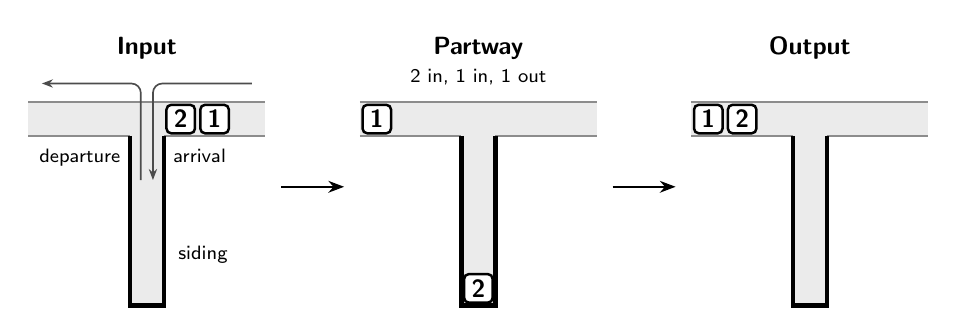
\begin{tikzpicture}[x=1mm,y=1mm]
\begin{scope}[shift={(12.9,0)}]
\fill[black!8] (-12.9,0) rectangle (17.2,4.3);
\fill[black!8] (0,-21.5) rectangle (4.3,0);
\draw[black!45, line width=0.5pt] (-12.9,4.3) -- (17.2,4.3);
\draw[black!45, line width=0.5pt] (-12.9,0) -- (0,0);
\draw[black!45, line width=0.5pt] (4.3,0) -- (17.2,0);
\draw[line width=1.6pt] (0,0) -- (0,-21.5) -- (4.3,-21.5) -- (4.3,0);
\draw[line width=0.9pt, fill=white, rounded corners=0.6mm] (4.64,0.34) rectangle (8.26,3.96);
\node at (6.45,2.15) {\bfseries\small 2};
\draw[line width=0.9pt, fill=white, rounded corners=0.6mm] (8.94,0.34) rectangle (12.56,3.96);
\node at (10.75,2.15) {\bfseries\small 1};
\node[font=\scriptsize, below left, inner xsep=1pt] at (-0.8,-0.4) {departure};
\node[font=\scriptsize, below right, inner xsep=1pt] at (5.1,-0.4) {arrival};
\node[font=\scriptsize, right] at (4.9,-15.05) {siding};
\draw[-{Stealth[length=1.4mm]}, line width=0.6pt, black!70, rounded corners=1.2mm] (15.48,6.67) -- (2.92,6.67) -- (2.92,-5.59);
\draw[-{Stealth[length=1.4mm]}, line width=0.6pt, black!70, rounded corners=1.2mm] (1.38,-5.59) -- (1.38,6.67) -- (-11.18,6.67);
\node[font=\small\bfseries] at (2.15,11.18) {Input};
\end{scope}
\draw[-{Stealth[length=2mm]}, line width=0.8pt] (32.1,-6.45) -- (40.1,-6.45);
\begin{scope}[shift={(55,0)}]
\fill[black!8] (-12.9,0) rectangle (17.2,4.3);
\fill[black!8] (0,-21.5) rectangle (4.3,0);
\draw[black!45, line width=0.5pt] (-12.9,4.3) -- (17.2,4.3);
\draw[black!45, line width=0.5pt] (-12.9,0) -- (0,0);
\draw[black!45, line width=0.5pt] (4.3,0) -- (17.2,0);
\draw[line width=1.6pt] (0,0) -- (0,-21.5) -- (4.3,-21.5) -- (4.3,0);
\draw[line width=0.9pt, fill=white, rounded corners=0.6mm] (-12.56,0.34) rectangle (-8.94,3.96);
\node at (-10.75,2.15) {\bfseries\small 1};
\draw[line width=0.9pt, fill=white, rounded corners=0.6mm] (0.34,-21.16) rectangle (3.96,-17.54);
\node at (2.15,-19.35) {\bfseries\small 2};
\node[font=\small\bfseries] at (2.15,11.18) {Partway};
\node[font=\scriptsize] at (2.15,7.52) {2 in, 1 in, 1 out};
\end{scope}
\draw[-{Stealth[length=2mm]}, line width=0.8pt] (74.2,-6.45) -- (82.2,-6.45);
\begin{scope}[shift={(97.1,0)}]
\fill[black!8] (-12.9,0) rectangle (17.2,4.3);
\fill[black!8] (0,-21.5) rectangle (4.3,0);
\draw[black!45, line width=0.5pt] (-12.9,4.3) -- (17.2,4.3);
\draw[black!45, line width=0.5pt] (-12.9,0) -- (0,0);
\draw[black!45, line width=0.5pt] (4.3,0) -- (17.2,0);
\draw[line width=1.6pt] (0,0) -- (0,-21.5) -- (4.3,-21.5) -- (4.3,0);
\draw[line width=0.9pt, fill=white, rounded corners=0.6mm] (-12.56,0.34) rectangle (-8.94,3.96);
\node at (-10.75,2.15) {\bfseries\small 1};
\draw[line width=0.9pt, fill=white, rounded corners=0.6mm] (-8.26,0.34) rectangle (-4.64,3.96);
\node at (-6.45,2.15) {\bfseries\small 2};
\node[font=\small\bfseries] at (2.15,11.18) {Output};
\end{scope}
\end{tikzpicture}

\end{center}
Ask ``Which car has to leave first?'' Car 2 is at the front, so it drives into the siding to wait; car 1 drives in on top of it and straight out to the departure track; then car 2 comes out. Show two illegal moves, lifting car 1 over car 2 and pulling car 2 out from under car 1, and ask the group to say ``stop'' at either; at the tables the partner does this job. Then hold up page~1 and its picture, the same action with \tr{1\,3\,2}, and say what the pages ask: which trains can leave 1, 2, 3, \dots{} in order; mark \yes{} if they can and \no{} if they cannot, however you try. Do not drive \tr{2\,3\,1} or any printed train, and do not say what makes a train stick.

\textbf{A first visit.} Allow 35--40 minutes at the tables; finishing every page is not the goal. \emph{K--1:} Problems~1--3 (about 10, 10--15 and 10 minutes), then Problem~5's partner game if time remains. Return visit: Problem~4, more of Problem~5, then Problem~6. \emph{Grades 2--3:} Problems~1--3, with Problem~2's shared cards taking 15--20 minutes; quick pairs begin Problem~4. Return visit: Problems~4--5, then 6--7. \emph{Grades 4--5:} Problems~1--3 (10--15 minutes each), with Problem~3 as a conversation about why the rule always works. A quick trio can drive only the five-car rows of Problem~2 and start Problem~4's grids; the long trains can test the rule later. Return visit: Problems~4--7 (paths and counts); Problem~8 can fill a third visit. In the closing share, one table shows a stuck train and says what traps which car.

\newpage
\head{Answers and hints}
\textbf{At every table.} When a pair marks \no{} after one try, ask ``Was there a moment when the car you needed was on top?'' When a child lifts or reaches past a car, ask the partner what the rule says. When an argument runs ahead of the cars, ask them to drive the train. Adult reading and recording are ordinary support; adult choice of moves means the task should shrink.

\head{Grades K--1}

\fbox{\parbox{\dimexpr\linewidth-2\fboxsep-2\fboxrule}{\textbf{Key in plain words for the K--1 adult.} A train is really stuck when a bigger car has to drive in on top of a smaller car while the car needed next has not arrived yet. Before accepting a \no, check that each needed car went out as soon as it was on top. Marks row by row, left box then right box: Problem~1: \yes~\yes{} / \yes~\no{} / \yes~\yes. Problem~2: \yes~\no{} / \yes~\yes{} / \no~\yes{} / \yes~\no. Problem~3: only \tr{4\,3\,2\,1} works. Problem~4: \no~\yes{} / \yes~\yes{} / \no~\no. Problem~6: 1342; 2314, 2341, 2413, 2431; 3142, 3241, 3412, 3421; 4231.}}

\sub{Problem 1, page 1: three cars}
Only \tr{2\,3\,1} is \no; the other five work, and \tr{1\,3\,2} is already pictured on page~1. Showing why with the cars: car 2 cannot leave before car 1, so it waits in the siding; car 3 cannot leave either, so it waits on top of 2; car 1 comes in and goes straight out; now car 2 is needed and car 3 sits on it. A child's explanation is pointing at that moment. Hint: ``Which car is on top? Which car do you need next?''

\sub{Problem 2, page 2: four cars}
\yes~\tr{2\,1\,4\,3}, \tr{4\,3\,2\,1}, \tr{1\,4\,3\,2}, \tr{3\,1\,2\,4}, \tr{4\,1\,3\,2}. \no~\tr{3\,4\,1\,2} (4 waits on 3), \tr{4\,2\,3\,1} (3 waits on 2), \tr{1\,3\,4\,2} (4 waits on 3). Hint: ``Which car is trapped, and which car is on top of it?'' Extension: one pair builds a stuck train for the other pair to explain.

\sub{Problem 3, page 3: car 1 last}
The six fillings are \tr{2\,3\,4\,1}, \tr{2\,4\,3\,1}, \tr{3\,2\,4\,1}, \tr{3\,4\,2\,1}, \tr{4\,2\,3\,1}, \tr{4\,3\,2\,1}; only \tr{4\,3\,2\,1} works. Since car 1 comes last, cars 2, 3 and 4 must all wait in the siding; to come out 2, 3, 4, car 2 must be on top and car 4 at the bottom, so they must arrive 4, 3, 2. The list is complete with two trains starting with each of 2, 3 and 4 and no repeats. Hint: ``Before car 1 comes, where are all the other cars?'' Extension: with five cars and car 1 last, only \tr{5\,4\,3\,2\,1} works.

\sub{Problem 4, page 4: five cars}
\yes~\tr{2\,1\,5\,4\,3}, \tr{5\,4\,3\,2\,1}, \tr{5\,1\,3\,2\,4}. \no~\tr{4\,5\,1\,2\,3} (5 waits on 4), \tr{1\,3\,5\,2\,4} (5 waits on 3), \tr{3\,2\,5\,1\,4} (5 waits on 2). \tr{5\,4\,3\,2\,1} fills all five siding places; if five real cars do not fit, let the bottom one overhang the end line and tell the organizer. Hint: ``Which car has to wait at the bottom, and what lands on it?''

\sub{Problem 5, page 4: guess, then drive}
Good guessers look for a bigger car that will have to wait on a smaller one. Hint for the guesser: ``Which car has to wait first? What comes after it?''

\sub{Problem 6, page 5: all ten stuck trains}
Grouped by first car: \tr{1\,3\,4\,2}; \tr{2\,3\,1\,4}, \tr{2\,3\,4\,1}, \tr{2\,4\,1\,3}, \tr{2\,4\,3\,1}; \tr{3\,1\,4\,2}, \tr{3\,2\,4\,1}, \tr{3\,4\,1\,2}, \tr{3\,4\,2\,1}; \tr{4\,2\,3\,1}. Seven were met before (\tr{3\,4\,1\,2}, \tr{4\,2\,3\,1}, \tr{1\,3\,4\,2} in Problem~2 and four in Problem~3); the new ones are \tr{2\,3\,1\,4}, \tr{2\,4\,1\,3} and \tr{3\,1\,4\,2}. The page gives the number, so the work is finding them without repeats and checking each by driving. Reasons a child can give: a train starting with 1 or 4 acts like a three-car train (car 1 drives straight through; car 4 waits at the bottom until the end), so each has one stuck train, the \tr{2\,3\,1} picture again; a train starting with 2 works only if 1 comes next; one starting with 3 works only if 4 is last. Hints: ``Which trains starting with 4 have you tried?'' ``Did you find that one already?'' The adult may record while children find and drive.

\head{Grades 2--3}
\sub{Problem 1, page 1: three cars}
The six trains are \tr{1\,2\,3}, \tr{1\,3\,2}, \tr{2\,1\,3}, \tr{2\,3\,1}, \tr{3\,1\,2}, \tr{3\,2\,1}; only \tr{2\,3\,1} is \no. The list is complete with two trains starting with each car. Hint: ``Which car is trapped, and by which car?''

\sub{Problem 2, page 2: all 24 four-car trains}
14 can and 10 cannot. Can: \tr{1\,2\,3\,4}, \tr{1\,2\,4\,3}, \tr{1\,3\,2\,4}, \tr{1\,4\,2\,3}, \tr{1\,4\,3\,2}, \tr{2\,1\,3\,4}, \tr{2\,1\,4\,3}, \tr{3\,1\,2\,4}, \tr{3\,2\,1\,4}, \tr{4\,1\,2\,3}, \tr{4\,1\,3\,2}, \tr{4\,2\,1\,3}, \tr{4\,3\,1\,2}, \tr{4\,3\,2\,1}. Cannot: the ten in K--1 Problem~6. By first car the ``can'' pile has 5, 2, 2 and 5. If the pairs ask how to share the work or how to know none is missing, ask ``How many trains start with car 1? How do you know?'' Count the cards: 24, with no two alike.

\sub{Problem 3, page 2: five cars}
\yes~\tr{3\,2\,1\,5\,4}, \tr{4\,1\,3\,2\,5}, \tr{1\,2\,5\,3\,4}, \tr{5\,2\,1\,4\,3}. \no~\tr{2\,4\,3\,5\,1} (2, 4, 1), \tr{4\,5\,3\,2\,1} (4, 5, 1), \tr{3\,1\,5\,4\,2} (3, 5, 2), \tr{1\,5\,3\,4\,2} (3, 4, 2). Each triple names a waiting car, the bigger car that first lands on it, and the car needed at that moment, which had not yet come; this is where a drive that sends each needed car out at once first goes wrong. Any middle, largest, smallest triple in the train is equally right, and a child looking at the stuck siding may name a different one. Hint: ``When the trouble starts, which car is waiting, and what is on top of it?''

\sub{Problem 4, page 3: what makes a train impossible}
A train is impossible exactly when some car is followed, later, by a bigger car and, later still, by a car smaller than the first: middle, big, small, like \tr{2\,3\,1}. In children's words: ``a big car has to sit on a smaller one that is still waiting.'' Tempting rules to test: ``a small number before a big one'' (\tr{1\,2\,3} works), ``car 1 at the end'' (\tr{3\,2\,1} works), ``three neighbours that go middle, big, small'' (\tr{3\,1\,4\,2} and \tr{2\,4\,3\,1} stick without such neighbours). Hint, with a stuck train on the table: ``Which car got trapped? Where were the trapped car and the car on top of it in the train?'' Follow-up: ``Does your rule ever call a good train stuck?''

\sub{Problem 5, page 3: decide, then drive}
\yes~\tr{1\,4\,2\,3\,5}, \tr{5\,4\,1\,3\,2}, \tr{2\,1\,5\,3\,4}. \no~\tr{4\,2\,5\,1\,3} (2, 5, 1), \tr{3\,4\,5\,2\,1} (3, 4, 1), \tr{5\,3\,4\,1\,2} (3, 4, 1), triples read as in Problem~3. A disagreement between a mark and the drive is the useful moment: whose rule needs changing, and how?

\sub{Problem 6, page 4: where car 5 can join}
Number the dashed boxes from the left. \tr{2\,1\,4\,3}: first, third and fifth (\tr{5\,2\,1\,4\,3}, \tr{2\,1\,5\,4\,3}, \tr{2\,1\,4\,3\,5}). \tr{4\,3\,2\,1}: first and last. \tr{1\,3\,2\,4}: first, second, fourth and last. \tr{3\,1\,2\,4}: first, fourth and last. Car 5 can go where every car on its left is smaller than every car on its right. Why: a bigger car before 5 and a smaller one after it make the stuck pattern with 5 as the big car; otherwise the cars before 5 all leave before it arrives, and car 5 waits at the bottom until the end. Hint: ``When car 5 is in the siding, which cars are under it, and do they need to leave first?''

\sub{Problem 7, page 4: how many five-car trains}
42. \emph{From the Problem~2 pile:} taking car 5 out of a working train leaves a working four-car train, and putting it back is a Problem~6 question, so add the allowed gaps over the 14 cards: \tr{1\,2\,3\,4} has 5; \tr{1\,2\,4\,3}, \tr{1\,3\,2\,4}, \tr{2\,1\,3\,4} have 4; \tr{1\,4\,2\,3}, \tr{1\,4\,3\,2}, \tr{2\,1\,4\,3}, \tr{3\,1\,2\,4}, \tr{3\,2\,1\,4} have 3; the five starting with 4 have 2; total 42. \emph{By where car 5 sits:} first 14, second 5, third 4, fourth 5, last 14. Either count is checked by its reasoning: each working train comes from exactly one card and one gap, or from exactly one position of car 5. Hints: ``Take car 5 out of a train that works. Does the rest still work?'' ``Which of your 14 cards lets car 5 in the most places?'' Extension: six cars, with a paper car 6 and the siding treated as long enough: 132 (by where car 6 sits, $42+14+10+10+14+42$). On the five-place mat \tr{6\,5\,4\,3\,2\,1} cannot leave, which gives 131.

\head{Grades 4--5}
\sub{Problem 1, page 1: three cars, then the count of four}
Only \tr{2\,3\,1} is \no; 14 of the 24 four-car trains leave in order (listed under Grades 2--3 Problem~2). Two checks: by first car 5, 2, 2, 5; by the position of car 4, also 5, 2, 2, 5, since car 4 first or last leaves a three-car train (5 ways), and in the middle it forces 1 before it and 2, 3 after, or 1, 2 before and 3 after (2 ways each). Expect 10--15 minutes. If the trio wants to share the 24, ask how to split them so that nobody repeats a train; splitting by first car keeps each share checkable (5, 2, 2, 5 work). Hint: ``What does car 4 do in a train that works?''

\sub{Problem 2, page 2: longer trains}
\yes~\tr{3\,1\,2\,5\,4}, \tr{5\,1\,4\,2\,3}, \tr{1\,7\,2\,6\,3\,5\,4}, \tr{3\,2\,1\,7\,6\,4\,5}, \tr{4\,3\,1\,2\,8\,5\,7\,6}. \no~\tr{2\,4\,1\,5\,3} (2, 4, 1), \tr{1\,3\,5\,4\,2} (3, 5, 2), \tr{3\,6\,1\,2\,4\,5} (3, 6, 1), \tr{2\,1\,4\,6\,3\,5} (4, 6, 3), \tr{4\,1\,3\,2\,8\,6\,7\,5} (6, 7, 5). Driven by the never-fails rule, no train needs more than four places. The last pair differ in a few cars; ask why one sticks.

\sub{Problem 3, page 2: a rule and why it always works}
No middle--largest--smallest triple (Theorem 1). A full explanation has two halves. That a triple blocks is within reach: when the smallest car arrives, the other two are both waiting, the bigger on top. That no triple means success needs the first-trouble argument: suppose the never-fails drive must park a car on a smaller waiting car; at the first such moment, where is the car you need? Use that question only when children have the first half. Follow-up: ``How do you know no cleverer drive rescues a train with a triple?''

\sub{Problem 4, page 3: the fourteen paths}
U is a step up (car in), D a step down (car out); the worked \tr{1\,3\,2} is UDUUDD.
\begin{center}\small
\begin{tabular}{ll@{\qquad}ll@{\qquad}ll}
\tr{1\,2\,3\,4} & UDUDUDUD & \tr{1\,4\,3\,2} & UDUUUDDD & \tr{4\,1\,2\,3} & UUDUDUDD\\
\tr{1\,2\,4\,3} & UDUDUUDD & \tr{2\,1\,3\,4} & UUDDUDUD & \tr{4\,1\,3\,2} & UUDUUDDD\\
\tr{1\,3\,2\,4} & UDUUDDUD & \tr{2\,1\,4\,3} & UUDDUUDD & \tr{4\,2\,1\,3} & UUUDDUDD\\
\tr{1\,4\,2\,3} & UDUUDUDD & \tr{3\,1\,2\,4} & UUDUDDUD & \tr{4\,3\,1\,2} & UUUDUDDD\\
 & & \tr{3\,2\,1\,4} & UUUDDDUD & \tr{4\,3\,2\,1} & UUUUDDDD
\end{tabular}\end{center}
The page's 14 grids match Problem~1's count. Hint: ``In the \tr{1\,3\,2} example, which moves make the path go up?''

\sub{Problem 5, page 4: from path to train}
Top row \tr{1\,5\,3\,2\,4} and \tr{5\,2\,1\,4\,3}; bottom row \tr{4\,1\,3\,2\,5} and \tr{5\,3\,2\,1\,4}. Each down-step is the next car out (1, then 2, \dots), and it is the car that went in at the latest up-step not yet used. Hint: ``Which car is the first to come out? At which up-step did it go in?'' Fallback for a child still stuck after the hint: letter five of the blank paper squares A to E, follow the path on the mat (up, the front car goes in; down, the top car comes out), and give each car the next number as it leaves; the train is A's number, B's number, and so on.

\sub{Problem 6, page 4: is the path code one-to-one?}
No train has two drives: every move is forced (Theorem 2). No two trains share a path: the path says at which up-step each departing car entered, which rebuilds the train. The paths that come from trains are exactly those that never go below the start line, 14 of the 70 orders of four ups and four downs. The lattice has no dots below the line, so the real question is whether every such path comes from a train: decode it, and that train follows the path. Hint: ``What would a step below the line mean on the mat?''

\sub{Problem 7, page 5: 42 and 132}
Any one organized argument is a complete answer. \emph{Paths:} write at each dot the number of paths from the start that reach it without going below the line; each dot is the sum of the dots up-left and down-left; the final dot reads 42, or 132 for six. \emph{Largest car, or first car:} by the position of the largest car, $14+5+4+5+14=42$ and $42+14+10+10+14+42=132$; counting by the first car's number gives the same terms (in path language, the first car's number says when the path first returns to the line, Week~12's first-return split). \emph{Insertion}, as in Grades 2--3 Problem~7. The rules' long siding matters: with five places \tr{6\,5\,4\,3\,2\,1} could not leave, giving 131. Hints: ``How many paths reach each dot?'' ``Where can car 6 sit in a train that works?''

\sub{Problem 8, page 5: two sidings}
All three trains leave in order. One way: let the first siding turn the train into one that counts down, which the second siding then sorts. \tr{2\,3\,1}: first siding 2 in, 3 in, 3 out, 2 out, 1 in, 1 out, so \tr{3\,2\,1} travels on. \tr{3\,4\,1\,2} can become \tr{4\,3\,2\,1} (3 in, 4 in, 4 out, 3 out, 1 in, 2 in, 2 out, 1 out), and \tr{2\,5\,3\,4\,1} becomes \tr{5\,4\,3\,2\,1} (2 in, 5 in, 5 out, 3 in, 4 in, 4 out, 3 out, 2 out, 1 in, 1 out). Two-siding drives are not unique, so other answers are right too.

Seven cars: yes, 22 trains fail, such as \tr{2\,4\,3\,5\,7\,6\,1}; all end in car 1. Children will most likely find that everything they try works and conjecture ``no'' (see Theorem~4). Treat that as good evidence for a false conjecture, then offer \tr{2\,4\,3\,5\,7\,6\,1} as a challenge. Hint: ``Car 1 comes last. Which cars can leave the first siding before it arrives, and in what order?''

\emph{Why \tr{2\,4\,3\,5\,7\,6\,1} fails (for the adult).} The first siding's output must have no 2-3-1. Cars sent on before car 1 arrives must go in decreasing order (two increasing ones, then car 1, make a 2-3-1); the rest follow car 1, top first. \emph{If car 2 goes before car 1 arrives,} it is the last to go then and leaves an empty siding. Car 5 cannot go early: 4 and 3 would go too, after it, with 3 on top of 4. So 5, 7 and 6 arrive later, stay, and follow car 1 as 6, 7, 5, a 2-3-1. \emph{If car 2 stays,} it comes out last. Every early car must exceed every other stayer (early $b$, a bigger stayer, then 2 is a 2-3-1), and the stayers must come out decreasing, so they entered increasing. Since 4 arrives before 3, the stayers are $\{2\}$ or $\{2,3\}$. Either way 4 goes early, after 7, 6 and 5, so 3 lands on top of 4 first: kept, it blocks 4; sent early, it goes before 4, out of order.

\head{Sources and use}
Donald E. Knuth, \emph{The Art of Computer Programming}, vol.~1, 3rd ed.\ (1997), \S2.2.1, exercises 2--5 (the railway with a siding, the 2-3-1 condition and the count). Robert E. Tarjan, ``Sorting using networks of queues and stacks'', \emph{Journal of the ACM} 19 (1972), 341--346 (several sidings). Both references are as recorded in the theme's outline; neither book nor paper is in this checkout, so their exercise and page numbers were not checked, and nothing here is copied from them. The proofs, examples and counts above were written for this guide and checked independently by computer. Library connections: Week~12 (Catalan bijections: mountain paths and the first-return split), Week~23 (sorting with fixed comparator bars), Week~3 (orders as permutations).

Record what children tried and which questions they wanted to continue: whether partners kept cars in line, how often a good train was marked \no{} after one wrong move, whether K--1 children could say what traps a car, and whether five cars fit the siding.
\end{document}
